\documentclass[12pt]{article}
\usepackage[utf8]{inputenc}
\usepackage{amsmath}
\usepackage{mathrsfs}
\usepackage{amssymb}
\usepackage{amsfonts}

\DeclareMathOperator{\logit}{logit}
\DeclareMathOperator*{\argmax}{arg\,max}
\DeclareMathOperator*{\argmin}{arg\,min}
\newcommand{\red}[1]{\textcolor{red}{#1}}

\usepackage[
    a4paper,
    left = 2.5cm,
    right = 2.5cm,
    top = 2.5cm,
    bottom = 2.5cm
]{geometry}

\usepackage{graphicx}
\usepackage{booktabs}
\usepackage[headings]{fullpage}
\usepackage{xcolor}
\usepackage{hyperref}
\usepackage{fancyhdr}
 %For aligned formulas
 \usepackage{IEEEtrantools}
\usepackage{listings} %Source code listings https://en.wikibooks.org/wiki/LaTeX/Source_Code_Listings

% \lstset{
%     language=R, %You can always set to another language
%     breaklines,
%     deletekeywords={category},
%     basicstyle=\ttfamily\footnotesize,
%     otherkeywords={!,!=,~,\$,*,\&,\%/\%,\%*\%,\%\%,<-,<<-},
%     literate={~}{$\sim$}1 {<-}{{$\gets$}}1
% }

\usepackage[
    backend=biber,
    style=apa,
    maxcitenames=2,
    mincitenames=1,
    sorting=ynt
    ]{biblatex}
\addbibresource{bibfile.bib}

\setlength{\headheight}{15pt}
\pagestyle{fancy}
\fancyhf{}
\rhead{Odole, Cunha, and Murthy} % Fill in your name
%\lhead{Bayesian Statistics \& Probabilistic Machine Learning---Project Report}
\rfoot{Page \thepage}


\begin{document}

\begin{titlepage}
        \centering % Center all text
        \vspace*{\baselineskip} % White space at the top of the page
        
        {\huge YOUR TITLE}\\[0.2\baselineskip] % Title
        
        
        \vspace*{\baselineskip}
        
        {\Large --- Project Report ---\\
          Advanced Bayesian Data Analysis\\[\baselineskip]} % Tagline(s) or further description
        \vspace*{\baselineskip}
        
        {\LARGE Eldaleona Odole,  Leonor Cunha, and Anarghya Murthy\\[\baselineskip]} % Editor list  
        
        \vspace*{\baselineskip}

        \vfill
        
        \today \par % Location and year
        
        \vspace*{\baselineskip}

        {\itshape TU Dortmund University\par} % Editor affiliation
    \end{titlepage}

\clearpage

% \section{Template}
% This is a template for the project report in the course Advanced Bayesian Data Analysis.
% Fill in your title and names for the title page and header and follow the general structure. You don't have to use multiple chapters or sections at all for this short report, but if you do, don't go further than subsections--- \textcite{feynman1963lnphysics} didn't need to\ldots

% Some examples on how to use \LaTeX{} are shown below. If you want to reference something, you can do it as so:
% \textcite{mcelreath2016statistical}.

% \subsection{Images}
% \begin{figure}
%     \begin{center}
%     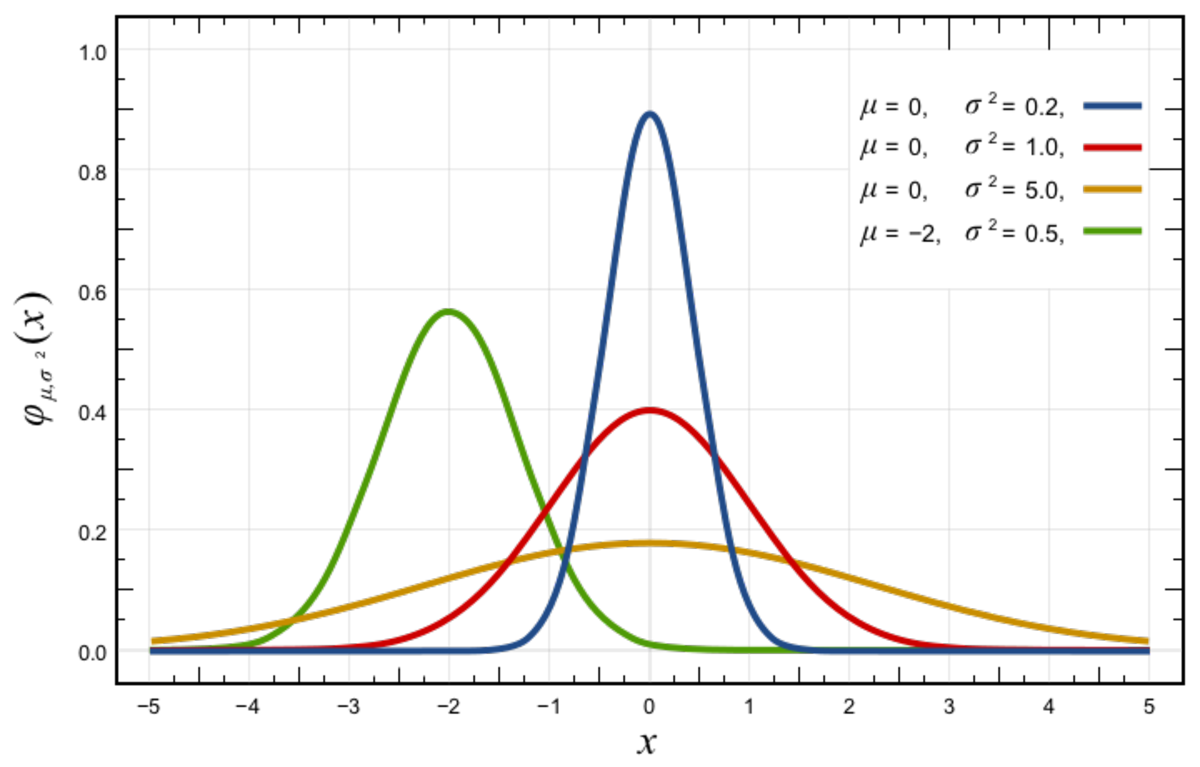
\includegraphics[width=0.5\textwidth]{figures/Normal_Distribution_PDF.pdf} %try to never force a figure placement
%     \caption{Probability density function for the Normal distribution. The red curve is the standard normal distribution. [By Inductiveload - self-made, Mathematica, Inkscape, Public Domain, \url{https://commons.wikimedia.org/w/index.php?curid=3817954}]}
%     \label{fig:normal_sample}
%     \end{center}
% \end{figure}

% This is an example for how to insert images into your document. When talking about a figure, you should always point out which one you mean, i.e., ``As you can see in Figure~\ref{fig:normal_sample}.''

% \subsection{Tables}
% A table has a caption \textit{above} the table as in Table~\ref{tab:my_label}.

% \begin{table} %You can place [h] immediately after \begin{table} to force the placement of the table. Generally speaking never do that---LaTeX usually places them in a sane way!
%     \centering
%     \caption{My caption.}
%     \label{tab:my_label}
%     \begin{tabular}{c|l} % l, r, and c justified inside cells.
%         \hline
%          Poisson & $\lambda$ \\ % Always end a line with \\
%          Normal &  $\mu$ and $\sigma$\\ 
%         \hline
%     \end{tabular}
% \end{table}

% \subsection{Formulas}
% This is a small example for how to include formulas into your document. $a^2 + b^2 = c^2$ will inline a formula, while
% $$c \leq a + b$$
% will give the formula its own line.

% \subsection{Formulas}
% You also might want to write out models:

% {\footnotesize % you align formulas using & 
% \begin{IEEEeqnarray*}{rCl}
% \mathrm{L}_i & \sim & \mathrm{Binomial}(n_i,p_i)\\
% \mathrm{logit}(p_i) & = & \alpha_{\mathrm{SUBJECT}[i]} + (\beta_P + \beta_{PC}C_i)P_i\\
% \alpha_{\mathrm{SUBJECT}} & \sim & \mathrm{Normal}(0,10) \\
% \beta_P & \sim & \mathrm{Normal}(0,10)\\
% \beta_{PC} & \sim & \mathrm{Normal}(0,10)
% \end{IEEEeqnarray*}
% }


% \subsection{Source code}
% Of course, formatting source code is always nice.
% \begin{lstlisting}
% m <- map(
%     alist(
%         height ~ dnorm(mu, sigma),
%         mu <- a + b*weight,
%         a ~ dnorm(0, 100),
%         b ~ dnorm(0, 10),
%         sigma ~ dunif(0, 50) 
%     ), 
%     data=d2)
% \end{lstlisting}

% \subsection{Math fonts}
% Different math fonts are also available to you:

% $\mathrm{ABCDE abcde 1234}$

% $\mathit{ABCDE abcde 1234}$

% $\mathnormal{ABCDEabcde1234}$

% $\mathcal{ABCDE abcde 1234}$

% $\mathscr{ABCDE abcde 1234}$

% $\mathfrak{ABCDE abcde 1234}$

% $\mathbb{ABCDE abcde 1234}$

\section{Introduction}


\textcolor{red}{notes to ourselves about things that should go in each section can be in red like this so we dont forget to delete them :)}


\subsection{Background}
The association between a voters demographics (gender, age, education etc.) and their propensity to vote for either a democratic or republican candidates is a topic of extensive study. The large political polling organization such as Gallup and \textcolor{red}{other org} tend to analyze their polls by breaking respondants into smaller demographic groups. However, less is known about the relationship between voting outcomes and the voter's environment. Our modeling would like to investigate the conventional wisdom that says cities tend to be more progressive. To put it more concreatly we want to investigate the question; "How does urbanization of a particular US House distrcit affect the resulting party that is elected?". 

To answer our question about the nature of the relationship between urbanizaiton and partisan voting outcomes, we choose to investigate the 2022 House Election. Every two years the United States elects 435 officials to the House of Representatives. Each state is allocated one of the the 435 House seats with the rest being allocated roughly proportional to the share of total population living in each state. When then use each one the districts as a single replicate since they are approximately equivalent in population size, but the characteristics of voters living in each district varies.

% Previous attempts? 

Inherent in our analysis is the assumption that voters for each are not evenly distributed, rather we assume that the distribution of voters is informative for our analysis. Much of the current research related to the relationship between urbanization and partisan voting focuses on the practice of gerrymandering. Gerrymanding is practice of redrawing the voting district boundaries in favor of a particular political party. We ignore the impact of gerrymandering in our analysis, and assume that the districts are drawn fairly.

As we are using a custom dataset it was difficult to find directly comparable research, however we did find interesting ideas related to urbanization and partisianship. One example of this would be the idea of the inefficent distribution of Democrats in cities, as explored by \textcolor{red}{CITE}. In their analysis they show that Democrats tend to more often be located quite densly in the urban core or surrounding nearby suburbs of a city, whereas Republicans tend to live further from city centers. Rather than trying to predict the partisan outcome of a particular district, their analysis focuses on describing partisal spatial efficency. \textcolor{red}{what is partisan spatial efficency/inefficency?}
This is related to our analysis because where these authors were trying to understand the outcomes as related to distribution of voters within a city we are tyring to do somehting similar but rather look to predicting the outcomes of particular districts with respect to their level of urbanization. Whereas the authors assume some sort of causal mechanism in the urbanization being a determinate variable for partisanship be assume rather that both partisanship and urbanization are independent given some other third latent variable. 


\textcolor{red}{conclusions of the introduction or somehing basically }
The 2022 House Election takes places during a non-presidential year, and is the most recent election following the 2020 Census and redistricting, allowing us to use the most recently available district maps, and demographic data. Within this report we combine demographic data and urbanization data into a logistic regression model to predict the district voting outcomes of the 2022 House Election. 

\textcolor{red}{this is something like assumptions but im not really sure what to say}
Since the districts are allocated based on population, they are approximately the same size, which allows us the make the assumption the differences in voting behavior have something do with people within the districts rather than simply the size of each district. This also allows us the make exchangability assumptions with respect to state and region.




\section{Dataset}
Our dataset was made by combining four independent datasets related to the 2022 House election. The first dataset is the publically available urbanization dataset published by fivethirty eight from which we incorporate the variables urbanization index  and (urban) grouping into our final dataset \cite{urbanizationdataset}. From the description of the dataset: "The urbanization index is calculated as the natural logarithm of the average number of people living within a five-mile radius of every census tract in a given district, based on a weighted average of the population of each census tract. The population of a census tract is according to 2020 census data. This provides a numerical value for how urban or rural a district is. " \cite{urbanizationdataset}. The urbanization dataset was put together by FiveThirtyEight as part of their analysis  \textit{The Republican Path To a House Majority Goes Through The Suburbs} which gave election predictions leading up to the 2022 U.S. Congressional Eleciton \cite{538urbanizationarticle}. 
% maybe add something about this analysis? 

The second dataset used in our analysis the Election Results Dataset from FiveThirtyEight \cite{electionresultsdataset}. It is a continuously updated repository of United States Govenor, Congressional and Presidential elections. As this dataset includes all elections going back to 1998, we only used a subset of the data relevant to the 2022 House Election. From this dataset we used the party, state, and winner variables. 

The third data used in our analysis is a subset of the 2022 American Commuity Survey Data. The American Community Survey is a yearly survey collecting information about the occupations, education attainment, income and other demographic information carried out by the United States Census Bureau. The United States Census Bureau provides an online tool to access its extensive survey database, which can then be filtered and refined for further analysis. For our analysis we used the following variables for each House district; 

\textcolor{red}{add variables that we used}

The fourth dataset was the region dataset, which was put together manually by us following the region designations of \textcolor{red}{I forgot where we got this info tbh}

\subsection{Data Cleaning}

Since we used four different data sources, this meant merging different datasets on shared variables. As previously said, each observation represents a particular house district, so for the first three dataset, we simply merged them based on their state and district number. To include the regions we simply used the state variable for each district. 

In terms of scaling we wanted all the variables to be on roughly the same scale to aid in convergence times. In order to do that we roughly scaled median income and total population by dividing total population by one million and dividing median income by one hundred thousand. This brought each of these to roughly the same scale as the other variables that are in the range of zero to one as they are percentages. 

\section{Models}

%To describe our approach we wanted to test different models that incorporate the geographical hierarchy into the model. We made several common assumptions for the the four models that we compared with addtional more specific assumptions for each model. The first common assumption we made was that district voting outcomes can be modeled via logistic regression. This assumption gets at the basic logic of our models. As we said previously the outcomes of any particular district electoral race is binary (democrat/republic) so it is most appropriate to choose a modeling technique that can model binary outcomes. 
%
%\textit{Why did we choose logisitic regression?}
%
%We then moved on to our assumptions about the parameters of the linear regression model within the logistic regression model. We also assume that geography is a characteristic of each district that can be modeled hierarchical. For that reason we assume that each district is exchangeable within each state and that each state is exchangeable within each region. We assume this because for complicated historical reasons certain regiions of the united states are more similar to eachother than others. For example the Southern United states tends to be more religious and religous people tend to vote more conservatively, as a result the parameter associated with region would likely be smaller or more negative as compared to other regions. 
%We also are assuming that in some regions the value of urban index is more informative than others, the logic being that a city in a rural area will likely have stronger signal than an city among a bunch of other cities. 
%
%We also 
%
%++++++++++++++++++++++++++++++++++++++++++++++
\subsubsection{Two party system}

\textcolor{red}{Leonor: here is an explaination for it being two parties, kinda long but yeah}
Although technically a multiparty system, the U.S. is often called a two party system due to the domination of the major political parties the Democrats and Republicans \textcolor{red}{(cite)}. These parties dominate particularly on the fedral level because political candidates are required to get a plurality of votes rather than a majority of votes which the two largest parties often reach. This is further reinforced as would be third-party voters, often vote for one of the two major parties so ensure their voice is heard, rather than using thier vote on a candidate unlikely to reach a plurality of votes \textcolor{red}{(cite)}. Within our dataset, there are no districts represented by a third-party candidate and as such we will refer to the U.S. as being a two party system, which led to using logistic regression as a natural choice for modeling. 

The Winning party in each congressional district race ($y_{i,j,k}$ for district $i$, state $j$, region $k$) can be modeled as the outcome of Bernoulli trial, since this is a binary variable: \textcolor{red}{NOTE ON HOW WE KNOW IT IS NOT A 2 PARTY SYSTEM EXCEPT THAT OOPS IT IS}
\begin{equation}
	y_{i,j,k} \sim Ber \left( \pi_{j,k} = logit^{-1}(\theta_{j,k})  \right)
\end{equation}
with probability of a Democrat win $\pi_{j,k}$ modeled as the inverse logit transform of $\theta_{j,k}$, a linear combination of our covariates. The inverse logit function converts real numbers into quantities between 0 and 1, and is therefore a standard way to model probabilities \textcolor{red}{cite}.


We tested four different models for $\theta_{j,k}$, which include different covariates in addition to out variable of interest (Urban index) and incorporate our data's hierarchical structure in different ways. Therefore, all four are Multilevel Bayesian (Logistic) Models, which require particular assumptions: \textcolor{red}{CITE} 
first, that a logistic regression accurately represents the relationship between the log-odds of a Democrat win and the explanatory variables, that is, $\theta_{j,k}$ and our covariates are linearly related; second, interchangeability, meaning that each district is exchangeable within each state and each state is exchangeable within each region; and third, that the value of urban index (and other covariates) in a district has a different effect depending on the state/region it belongs to.


The logistic relationship is a common assumption in the literature (\textcolor{red}{cite}).
We can assume interchangeability because for complicated historical reasons certain regiions of the united states are more similar to eachother than others. For example the Southern United states tends to be more religious and religous people tend to vote more conservatively, as a result the parameter associated with region would likely be smaller or more negative as compared to other regions. 
The idea behind the differing effect strength of urban index values per region is that a city in a rural area will likely have stronger signal than an city among a bunch of other cities. \textcolor{red}{[rewrite some of this paragraph]}



\subsubsection*{Model 1}

Model 1 is our most extensive model. Here we used urban index and 4 additional covariates plus an intercept to explain $\theta_{j,k}$.
Both the state and region hierarchies were included, but on different covariates. Urban index and median income effects vary by state, while the slope of percentage of bachelor's degrees varies by region. The intercept and the slopes of percentage of women and percentage of retirees were considered to have the same effect for all districts, hence were modeled non-hierarchically.



\begin{equation} \label{eq:mod1_uncentered}
	\begin{aligned}
		\theta_{j,k} = & \beta_0 + \beta_{women} \cdot \text{Pct\_Women} + \beta_{uncent \: urbindex, j} \cdot \text{Urban\_Index} \\
		               & + \beta_{uncent \: bsc,k} \cdot \text{Pct\_Bach.} \\
		               & + \beta_{uncent \: inc,j} \cdot \text{Median\_Income} + \beta_{ret} \cdot \text{Pct\_Retirees}
	\end{aligned}
\end{equation}



Equation \ref{eq:mod1_uncentered} describes our model conceptually. In order to have a specification more compatible with R syntax so we can fit our model with brms, we reformulate the model as Equation \ref{eq:mod1_centered}, with the group-level (state or region) centered around zero, following \textcolor{red}{cite brms book}

To better understand what happens in the backend when we want to fit this model with BRMS, it is helpful to rewrite the equation \ref{eq:mod1_uncentered} in terms of 'global' and 'hierarchical' effects.





\begin{equation} \label{eq:mod1_centered}
	\begin{aligned}
		\theta_{j,k} = & \beta_0 + \beta_{women} \cdot \text{Pct\_Women}                                                                              \\
		               & + \beta_{urbindex} \cdot \text{Urban\_Index} + \beta_{urbindex, j} \cdot \text{Urban\_Index}                                 \\
		               & + \beta_{bsc} \cdot \text{Pct\_Bachelor's} + \beta_{bsc,k} \cdot \text{Pct\_Bach.} + \beta_{inc} \cdot \text{Median\_Income} \\
		               & + \beta_{inc,k} \cdot \text{Median\_Income} + \beta_{ret} \cdot \text{Pct\_Retirees}
	\end{aligned}
\end{equation}

Note that although we are interested in hierarchically varying coefficients for certain variables, we nevertheless include a non-varying coefficient for the same variables, e.g. we have both a global coefficient as well as a state dependent coefficient for urban index. 

\subsubsection*{Model 2} 

For Model 2 we significantly reduced the number of variables. We kept only our variable of interest, urban index, and percentage of retirees \textcolor{red}{[why?????]}
Here, the geographical hierarchy was incorporated through a \textit{nested hierarchy} of districts within states within regions.
So, this model assumes that the effect of urbanindex ($\beta_{urb, j:k}$) depends on state $j$ and region $k$ through a prior with mean parameter $\beta_{urb, k}$, which in turn varies by region and depends on hyper-mean $\beta_{urb}$ (which has its own prior, with hyper-hyper-parameters). Equation \ref{eq:mod2_centered} specifies the model, with the centered around zero formulation. 
% Model equation
\begin{equation} \label{eq:mod2_centered}
	\begin{aligned}
		\theta_{j,k} =    &\beta_0 + \beta_{urb} \cdot \text{Urban\_Index} + \beta_{urb,k} \cdot \text{Urban\_Index} \\
		&+ \beta_{urb,j:k} \cdot \text{Urban\_Index} + \beta_{ret} \cdot \text{Pct\_Retirees}
	\end{aligned}
\end{equation}



%% Priors
%\[\beta_0 \sim \text{Normal}(0, 0.5)\]
%\[\beta_1 \sim \text{Normal}(0, 1); \beta_2 \sim \text{t}(1,-2,1)\]
%\[\beta_{1,j} \sim \text{Normal}(0, \sigma_j)\]
%\[\beta_{1,j:k} \sim \text{Normal}(0, \sigma_{j:k})\]
%\[ \sigma_j; \sigma_{j:k} \sim \text{Halfcauchy}(10)\]



\subsubsection*{Model 3}




\begin{equation} \label{eq:mod3_centered}
	\begin{aligned}
		\theta_{j} =    &\beta_0 + \beta_{urb} \cdot \text{Urban\_Index} + \beta_{urb,j} \cdot \text{Urban\_Index} \\
		&+ \beta_{ret} \cdot \text{Pct\_Retirees}
	\end{aligned}
\end{equation}





\subsubsection*{Model 4}




\begin{equation} \label{eq:mod4_centered}
	\begin{aligned}
		\theta_{k} =    &\beta_0 + \beta_{urb} \cdot \text{Urban\_Index} + \beta_{urb,k} \cdot \text{Urban\_Index} \\
		&+ \beta_{ret} \cdot \text{Pct\_Retirees}
	\end{aligned}
\end{equation}





\section{Priors}



\begin{table}[h]
	\resizebox{\textwidth}{!}{%
		\begin{tabular}{l|llll}
			\toprule
			              & \multicolumn{1}{c}{Model 1}                  & \multicolumn{1}{c}{Model 2}                  & \multicolumn{1}{c}{Model 3}              & \multicolumn{1}{c}{Model 4}              \\ \hline
			Intercept     & $\beta_0 \sim N(0, 10)$                      & $\beta_0 \sim N(0, 10)$                      & $\beta_0 \sim N(0, 10)$                  & $\beta_0 \sim N(0, 10)$                  \\
			Urban Index   & $\beta_{urb} \sim N(0,1)$                    & $\beta_{urb} \sim N(0,1)$                    & $\beta_{urb} \sim N(0,1)$                & $\beta_{urb} \sim N(0,1)$                \\
			              & $\beta_{urb, j} \sim N(0, \sigma_{urb,j}), $ & $\beta_{urb, k} \sim N(0, \sigma_{k}), $     & $\beta_{urb, j} \sim N(0, \sigma_{j}), $ & $\beta_{urb, k} \sim N(0, \sigma_{k}), $ \\
			              & $\sigma_{urb,j} \sim Gamma(2,5)$             & $\sigma_{k} \sim Halfcauchy(10)$             & $\sigma_{j} \sim Halfcauchy(10)$         & $\sigma_{k} \sim Halfcauchy(10)$         \\
			              &                                              & $\beta_{urb, j:k} \sim N(0, \sigma_{j:k}), $ &                                          &                                          \\
			              &                                              & $\sigma_{j:k} \sim Halfcauchy(10)$           &                                          &                                          \\
			Pct.retirees  & $\beta_{ret} \sim t(1,-2,1)$                 & $\beta_{ret} \sim t(1,-2,1)$                 & $\beta_{ret} \sim t(1,-2,1)$             & $\beta_{ret} \sim t(1,-2,1)$             \\
			pct.women     & $\beta_{urb} \sim N(0,1)$                    &                                              &                                          &                                          \\
			pct bsc       & $\beta_{bsc} \sim t(1,0,1)$                  &                                              &                                          &                                          \\
			              & $\beta_{bsc, k} \sim N(0, \sigma_{bsc,k}), $ &                                              &                                          &                                          \\
			              & $\sigma_{bsc,k} \sim Halfnormal(0,1)$        &                                              &                                          &                                          \\
			median income & $\beta_{inc} \sim N(0,1)$                    &                                              &                                          &                                          \\
			              & $\beta_{inc, j} \sim N(0, \sigma_{inc,j}), $ &                                              &                                          &                                          \\
			              & $\sigma_{inc,j} \sim Halfnormal(0,1)$        &                                              &                                          &                                          \\ \bottomrule
		\end{tabular}%
		}
		\caption{Prior summary table}
		\label{tab:priors}
\end{table}




%% Priors
%\[\beta_0 \sim \text{Normal}(0, 0.5)\]
%\[\beta_1, \beta_2 \sim \text{Normal}(0, 1); \beta_3 \sim \text{Cauchy(0,1)}\] 
%\[\beta_4 \sim \text{Normal}(0,1); \beta_5 \sim \text{t}(1,-1,1)\]
%
%
%\[\beta_{2,j} \sim \text{Normal}(0, \sigma_{\beta_{2,j}})\]
%
%\[\beta_{3,k} \sim \text{Normal}(0, \sigma_{\beta_{3,k}})\]
%
%\[\beta_{4,j} \sim \text{Normal}(0, \sigma_{\beta_{4,j}})\]
%
%\[\sigma_{\beta_{2,j}} \sim \text{Gamma}(2,5) \]
%
%\[\sigma_{\beta_{3,k}} \sim \text{Normal}(0,1) \]
%
%\[\sigma_{\beta_{4,j}} \sim \text{Normal}(0,1) \]




%For many of our parameters we picked Normal distributions [reasons]

For the intercept $\beta_0$ in Model 1 we set a Normal prior centered at zero with a large standard deviation. 
This represents a weakly informative prior, as we had no strong beliefs about the intercept value, nor does it have any straightforward interpretation in our model: it theoretically represents the (logit of the) probability of a Democrat win in a district with no urbanization at all, a median income of zero dollars, and 0\% of women, retirees and citizens with a bachelor's degree in the population; such a district is obviously nonexistent.
%our assumption that the probability of either party winning is roughly 50\% (corresponding to a $\theta_{j,k}$ of zero) when all other factors are absent. [wrong]





In Model 1, neither Pct.Women nor Pct.Retirees are modeled hierarchically. 


The percentage of women is roughly the same in every district, so we do not expect this covariate to have a strong effect on the probability of either party winning, i.e, we expect $\beta_{women}$ to be close to zero. So, we set a prior for this slope which is centered around zero and has little variability: a standard normal prior. 

The Percentage of retirees in each district negatively correlates with the probability of a Democrat winning, but we do not know how strong this effect ought to be. Therefore, for the prior on $\beta_{ret}$ we chose a distribution centered around a negative number, and with relatively heavy tails, reflecting our uncertainty. 



The effects of urban index, percentage of bachelor degrees, and median income are all parameterized in 2 hierarchical levels: an average slope across all districts, and a varying slope by group (State or Region), $\beta_{covariate,j}$ or $\beta_{covariate,k}$, which follows a Normal distribution centered at zero with standard deviation modeled at group level (by a hyperprior).

 
For the population-level component of the urbanindex slope we opted for a standard normal prior. We chose not to make assumptions on the sign of the effect of this variable, as it is this variable that we are interested in studying. So, we set comparatively less-informative priors on the parameters representing the effect of the index.


As we expected the population-level effects of both Median Income and Pct Bscs to be positive in some cases and negative in others, we picked symmetric priors for both $\beta_{bsc}$ and $\beta_{inc}$. We are, however, less sure about the average null effect of the Percentage of Bachelor degrees, so for this slope parameter we opted for a prior with 'fatter tails', the standard Cauchy distribution rather than the Normal one.


All group-level (zero-centered) priors are Normal, by brms specification \textcolor{red}{is there a reason???}

For the hyperparameters, we chose a half standard normal prior for both the standard deviations of $\beta_{bsc,k}$ and $\beta_{inc,j}$. This is a narrow distribution, with most values falling between 0 and 1, as we expect to see weak effects for these covariates, and thus small standard deviations (and positive, as any SD is by definition). For the standard deviation of $\beta_{urb,j}$, on the contrary, we opted for a less informative prior. Again, we do not want to make such strong assumptions about the effect of our variable of interest, hence we "allow the estimates to fluctuate more".






\section{Code}


\section{Results}

\textcolor{red}{This section is not on the instructions but is probably the easiest way to talk about the results we got }




\section{Convergence Diagnostics}

One of the fundamentals of Bayesian analysis is its reliance on MCMC sampling. This ensures we have access to both the posterior samples and (in our case) the posterior regression coefficients themselves. All our data analysis was done using BRMS, which runs on STAN, which itself uses the Hamiltonian Monte Carlo algorithm for the posterior generation. 

"Convergence " in layman's terms can be described as, 'Do the posterior draws get closer and closer to a specific value?'.

HMC Convergence diagnostics in itself can be a rather extensive topic, so for this project we only consider graphical and summary output based diagnostics, namely: the MCMC trace plots as provided by BRMS, and the Effective Sample Size as provided by the summary output command.

For the first model, we see that all 4 chains are relatively horizontal, and each chain appears to be 'centred' around a particular value. There are no divergent transitions for any coefficient for this model. 

\section{Model Comparison}


Our four models were built based on somewhat different assumptions about the structure of our data, and all produced slightly different results. We need to know which of these is \textit{better}, that is, which results are more trustworthy and allow us to answer our original research question.
To this end, we measured and compared our models' predictive performance first by looking at absolute predictive performance, then at relative and finally at the Leave-One-Out statistics to compare out-of-sample Predictive Performance.


To measure absolute predictive performance we used the Root Mean of Squared Error (RMSE)
\textcolor{red}{(FORMULA???)}.
This measure works in a similar way to the R squared statistic that is commonly used to assess the fit of linear models, by evaluating differences between observations and model predictions, but RMSE retains the scale of the response variable, meaning it has a direct interpretation in the context of our problem.
It takes into account the uncertainty of the posterior distribution by...


[plots of RMSE draws, overlap for comparison]

[interpretation]



To assess relative predictive performance, we looked at log-likelihood scores, that is, the average of posterior draws' log-likelihoods for each observation
\textcolor{red}{(FORMULA???)}. 
This is a relative predictive performance measure in the sense that it does not tell us anything about the model's predictive performance alone, we need to compare it between different models to establish which is better.
 

[plot of ll scores or likelihood differences?, overlap]

[interpretation]

%Note: these metrics are in-sample, so is biased towards more complex models 


In-sample predictive performance measures evaluate only model predictions for the same observations which were used to fit the model in the first place, therefore they tend to favor more complex models.
(In our case, the bigger mmodel (Model 1) was indeed the preferred one using both RMSE and LL scores.?????????????????')
Because we are comparing models with different degrees of complexity, it is essential to check also out-of-sample predictive performance metrics. These metrics are computed by splitting the dataset into training data and test data, fitting the model on the former and assessing the likelihood (ELPD) of the observations in the latter, given the model estimates with the training set.
\textcolor{red}{ELPD FORMULA??????????????}

The way we choose to split the data into training/test sets naturally impacts the ELPD. So, we rely on cross-validation: we do multiple different splits and average over the results. Our chosen method was Leave-One-Out cross-validation, which in theory performs as many splits as observations in the dataset, each time leaving one "out" as the test data. In practice, a different posterior is not actually computed this many times, but rather an estimate from the full model posterior using importance sampling (PSIS).

[LOO statistics table]

According to the LOO statistics, model 1 is the preferred one.

[pareto k estimates issue and momnet matching?]


\section{Prior Sensitivity Analysis}

\textcolor{red}{another table with priors here, maybe not all because thats a lot}

One of the most important parts of Bayesian Data Analysis is setting the prior distributions. The choice of priors could greatly affect the final results in a model..  \textcolor{red}{(cite prior sensitivity guys)}
So, we conducted a prior sensitivity analysis, by refitting our model(s) using alternative priors (which also fit our model assumptions) and assessing the impact in our results.

[BRIEFLY explain new priors, graphs comparing them]



\section{Limitations and Improvements}


\section{Conclusion}

\subsection{Reflection on own learnings}

\textcolor{red}{please lets call this subsection something else, this sounds so childish}


\printbibliography

\end{document}
